% Options for packages loaded elsewhere
\PassOptionsToPackage{unicode}{hyperref}
\PassOptionsToPackage{hyphens}{url}
%
\documentclass[
  ignorenonframetext,
]{beamer}
\usepackage{pgfpages}
\setbeamertemplate{caption}[numbered]
\setbeamertemplate{caption label separator}{: }
\setbeamercolor{caption name}{fg=normal text.fg}
\beamertemplatenavigationsymbolsempty
% Prevent slide breaks in the middle of a paragraph
\widowpenalties 1 10000
\raggedbottom
\setbeamertemplate{part page}{
  \centering
  \begin{beamercolorbox}[sep=16pt,center]{part title}
    \usebeamerfont{part title}\insertpart\par
  \end{beamercolorbox}
}
\setbeamertemplate{section page}{
  \centering
  \begin{beamercolorbox}[sep=12pt,center]{part title}
    \usebeamerfont{section title}\insertsection\par
  \end{beamercolorbox}
}
\setbeamertemplate{subsection page}{
  \centering
  \begin{beamercolorbox}[sep=8pt,center]{part title}
    \usebeamerfont{subsection title}\insertsubsection\par
  \end{beamercolorbox}
}
\AtBeginPart{
  \frame{\partpage}
}
\AtBeginSection{
  \ifbibliography
  \else
    \frame{\sectionpage}
  \fi
}
\AtBeginSubsection{
  \frame{\subsectionpage}
}
\usepackage{amsmath,amssymb}
\usepackage{iftex}
\ifPDFTeX
  \usepackage[T1]{fontenc}
  \usepackage[utf8]{inputenc}
  \usepackage{textcomp} % provide euro and other symbols
\else % if luatex or xetex
  \usepackage{unicode-math} % this also loads fontspec
  \defaultfontfeatures{Scale=MatchLowercase}
  \defaultfontfeatures[\rmfamily]{Ligatures=TeX,Scale=1}
\fi
\usepackage{lmodern}
\usecolortheme{beaver}
\usefonttheme{structurebold}
\ifPDFTeX\else
  % xetex/luatex font selection
\fi
% Use upquote if available, for straight quotes in verbatim environments
\IfFileExists{upquote.sty}{\usepackage{upquote}}{}
\IfFileExists{microtype.sty}{% use microtype if available
  \usepackage[]{microtype}
  \UseMicrotypeSet[protrusion]{basicmath} % disable protrusion for tt fonts
}{}
\makeatletter
\@ifundefined{KOMAClassName}{% if non-KOMA class
  \IfFileExists{parskip.sty}{%
    \usepackage{parskip}
  }{% else
    \setlength{\parindent}{0pt}
    \setlength{\parskip}{6pt plus 2pt minus 1pt}}
}{% if KOMA class
  \KOMAoptions{parskip=half}}
\makeatother
\usepackage{xcolor}
\newif\ifbibliography
\setlength{\emergencystretch}{3em} % prevent overfull lines
\providecommand{\tightlist}{%
  \setlength{\itemsep}{0pt}\setlength{\parskip}{0pt}}
\setcounter{secnumdepth}{-\maxdimen} % remove section numbering
\ifLuaTeX
  \usepackage{selnolig}  % disable illegal ligatures
\fi
\usepackage{bookmark}
\IfFileExists{xurl.sty}{\usepackage{xurl}}{} % add URL line breaks if available
\urlstyle{same}
\hypersetup{
  pdftitle={Political Inferences in the Wild: Inferring Politicians' Ideology from Apolitical Cues with Explicit Political Information. A visual conjoint approach},
  hidelinks,
  pdfcreator={LaTeX via pandoc}}

\title{Political Inferences in the Wild: Inferring Politicians' Ideology
from Apolitical Cues with Explicit Political Information. A visual
conjoint approach}
\author{Gaetano Scaduto\inst{1}, Fedra Negri\inst{1}, and Silvia
Decadri\inst{1}}
\date{2024 Workshop Survey Experiments in the Social Sciences. Amsterdam
Center for Inequality Studies (AMCIS). Amsterdam. 24 October 2024.}
\institute{\inst{1}University of Milan Bicocca,}

\begin{document}
\frame{\titlepage}

\begin{frame}{Introduction: A little anecdote}
\phantomsection\label{introduction-a-little-anecdote}
\begin{center}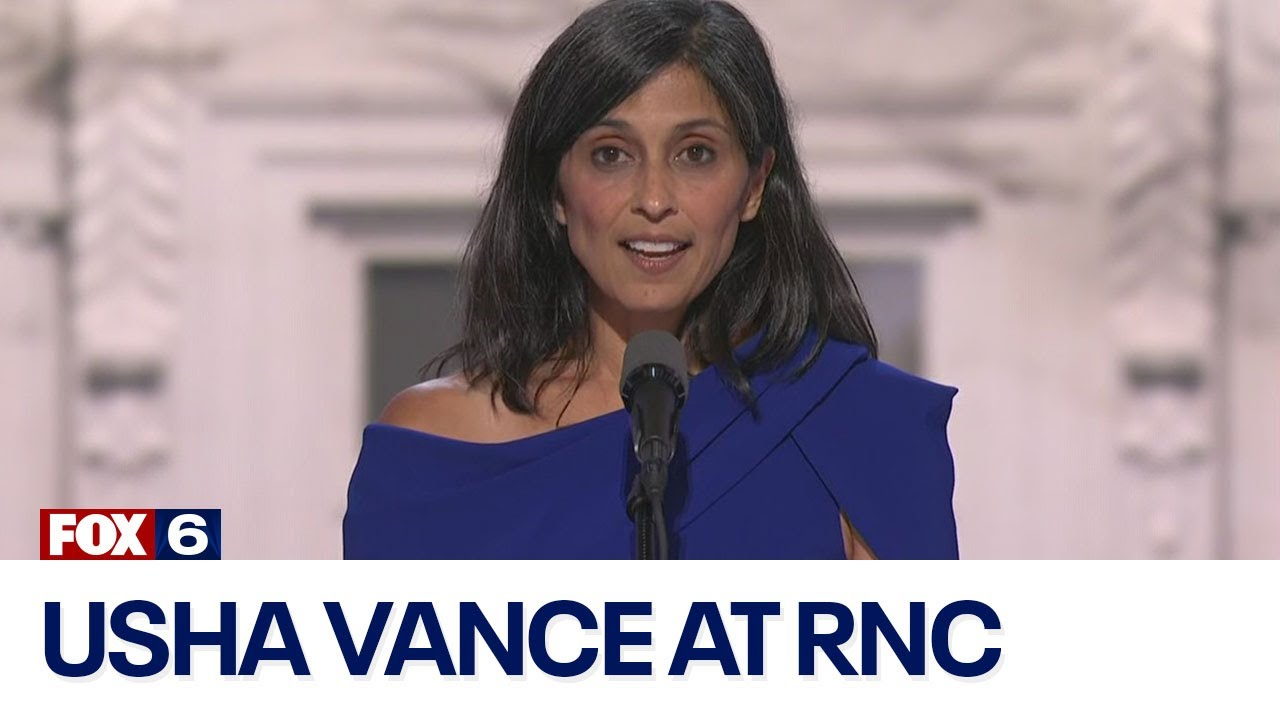
\includegraphics[width=1\linewidth]{../../visual_conjoint_experiment/Presentation/images/usha} \end{center}
\end{frame}

\begin{frame}{Theory 1/2}
\phantomsection\label{theory-12}
\begin{itemize}
\item
  Recent research has focused on the content and consequences of
  ``Political inferences from apolitical cues'' (Carlson \& Settle,
  2022; Lee, 2021; Scaduto \& Negri, 2024). These studies focused on
  what led people to form certain partisan or ideological expectations
  based on information that is not explicitly political.
\item
  Yet, these studies have focused on political inferences performed

  \begin{itemize}
  \tightlist
  \item
    On everyday partisans (but many studies also focused on
    politicians:, e.g.: Clifford 2020)
  \item
    In absence of explicitly political information
  \item
    In an unrealistic setting (survey experiments based on exclusively
    textual information)
  \end{itemize}
\end{itemize}
\end{frame}

\begin{frame}{Theory 2/2}
\phantomsection\label{theory-22}
\begin{itemize}
\tightlist
\item
  In this work we test whether there is a role of political inferences
  from apolitical cues:

  \begin{itemize}
  \tightlist
  \item
    Performed on politicians
  \item
    In presence of explicitly political information
  \item
    In a realistic setting
  \end{itemize}
\end{itemize}
\end{frame}

\begin{frame}{Research Questions}
\phantomsection\label{research-questions}
\begin{itemize}
\item
  RQ 1: Are political inferences from apolitical cues relevant for
  inferring politicians' left-right position? Apolitical cues:
  sociodemographic (gender, age, ethnicity, and occupation) or lifestyle
  (food and pet preferences)
\item
  RQ 2: Do apolitical cues keep their relevance also in presence of
  explicit political information, such a issue positions?
\end{itemize}
\end{frame}

\begin{frame}{Hypotheses}
\phantomsection\label{hypotheses}
\begin{center}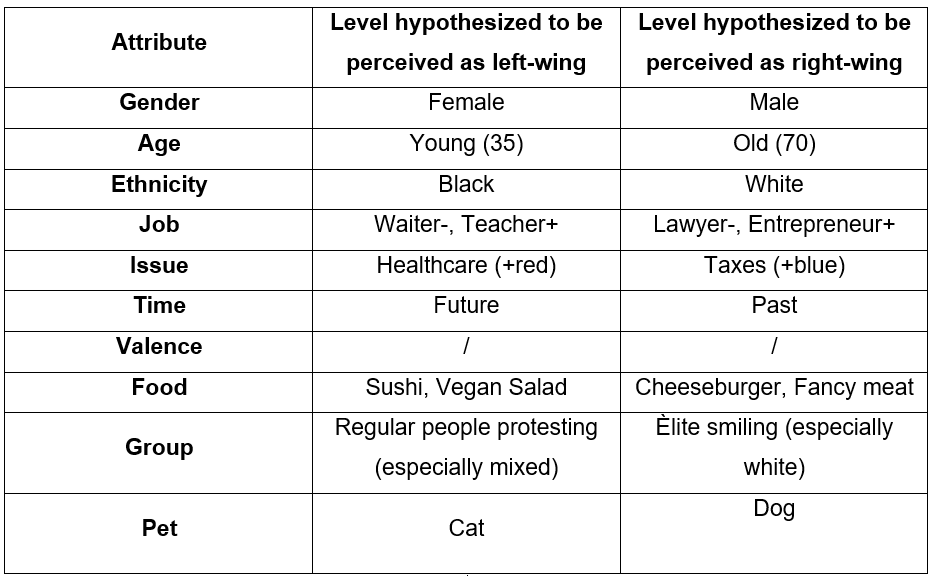
\includegraphics[width=0.9\linewidth]{../../visual_conjoint_experiment/Presentation/images/hyp} \end{center}
\end{frame}

\begin{frame}{Research Protocol}
\phantomsection\label{research-protocol}
\begin{center}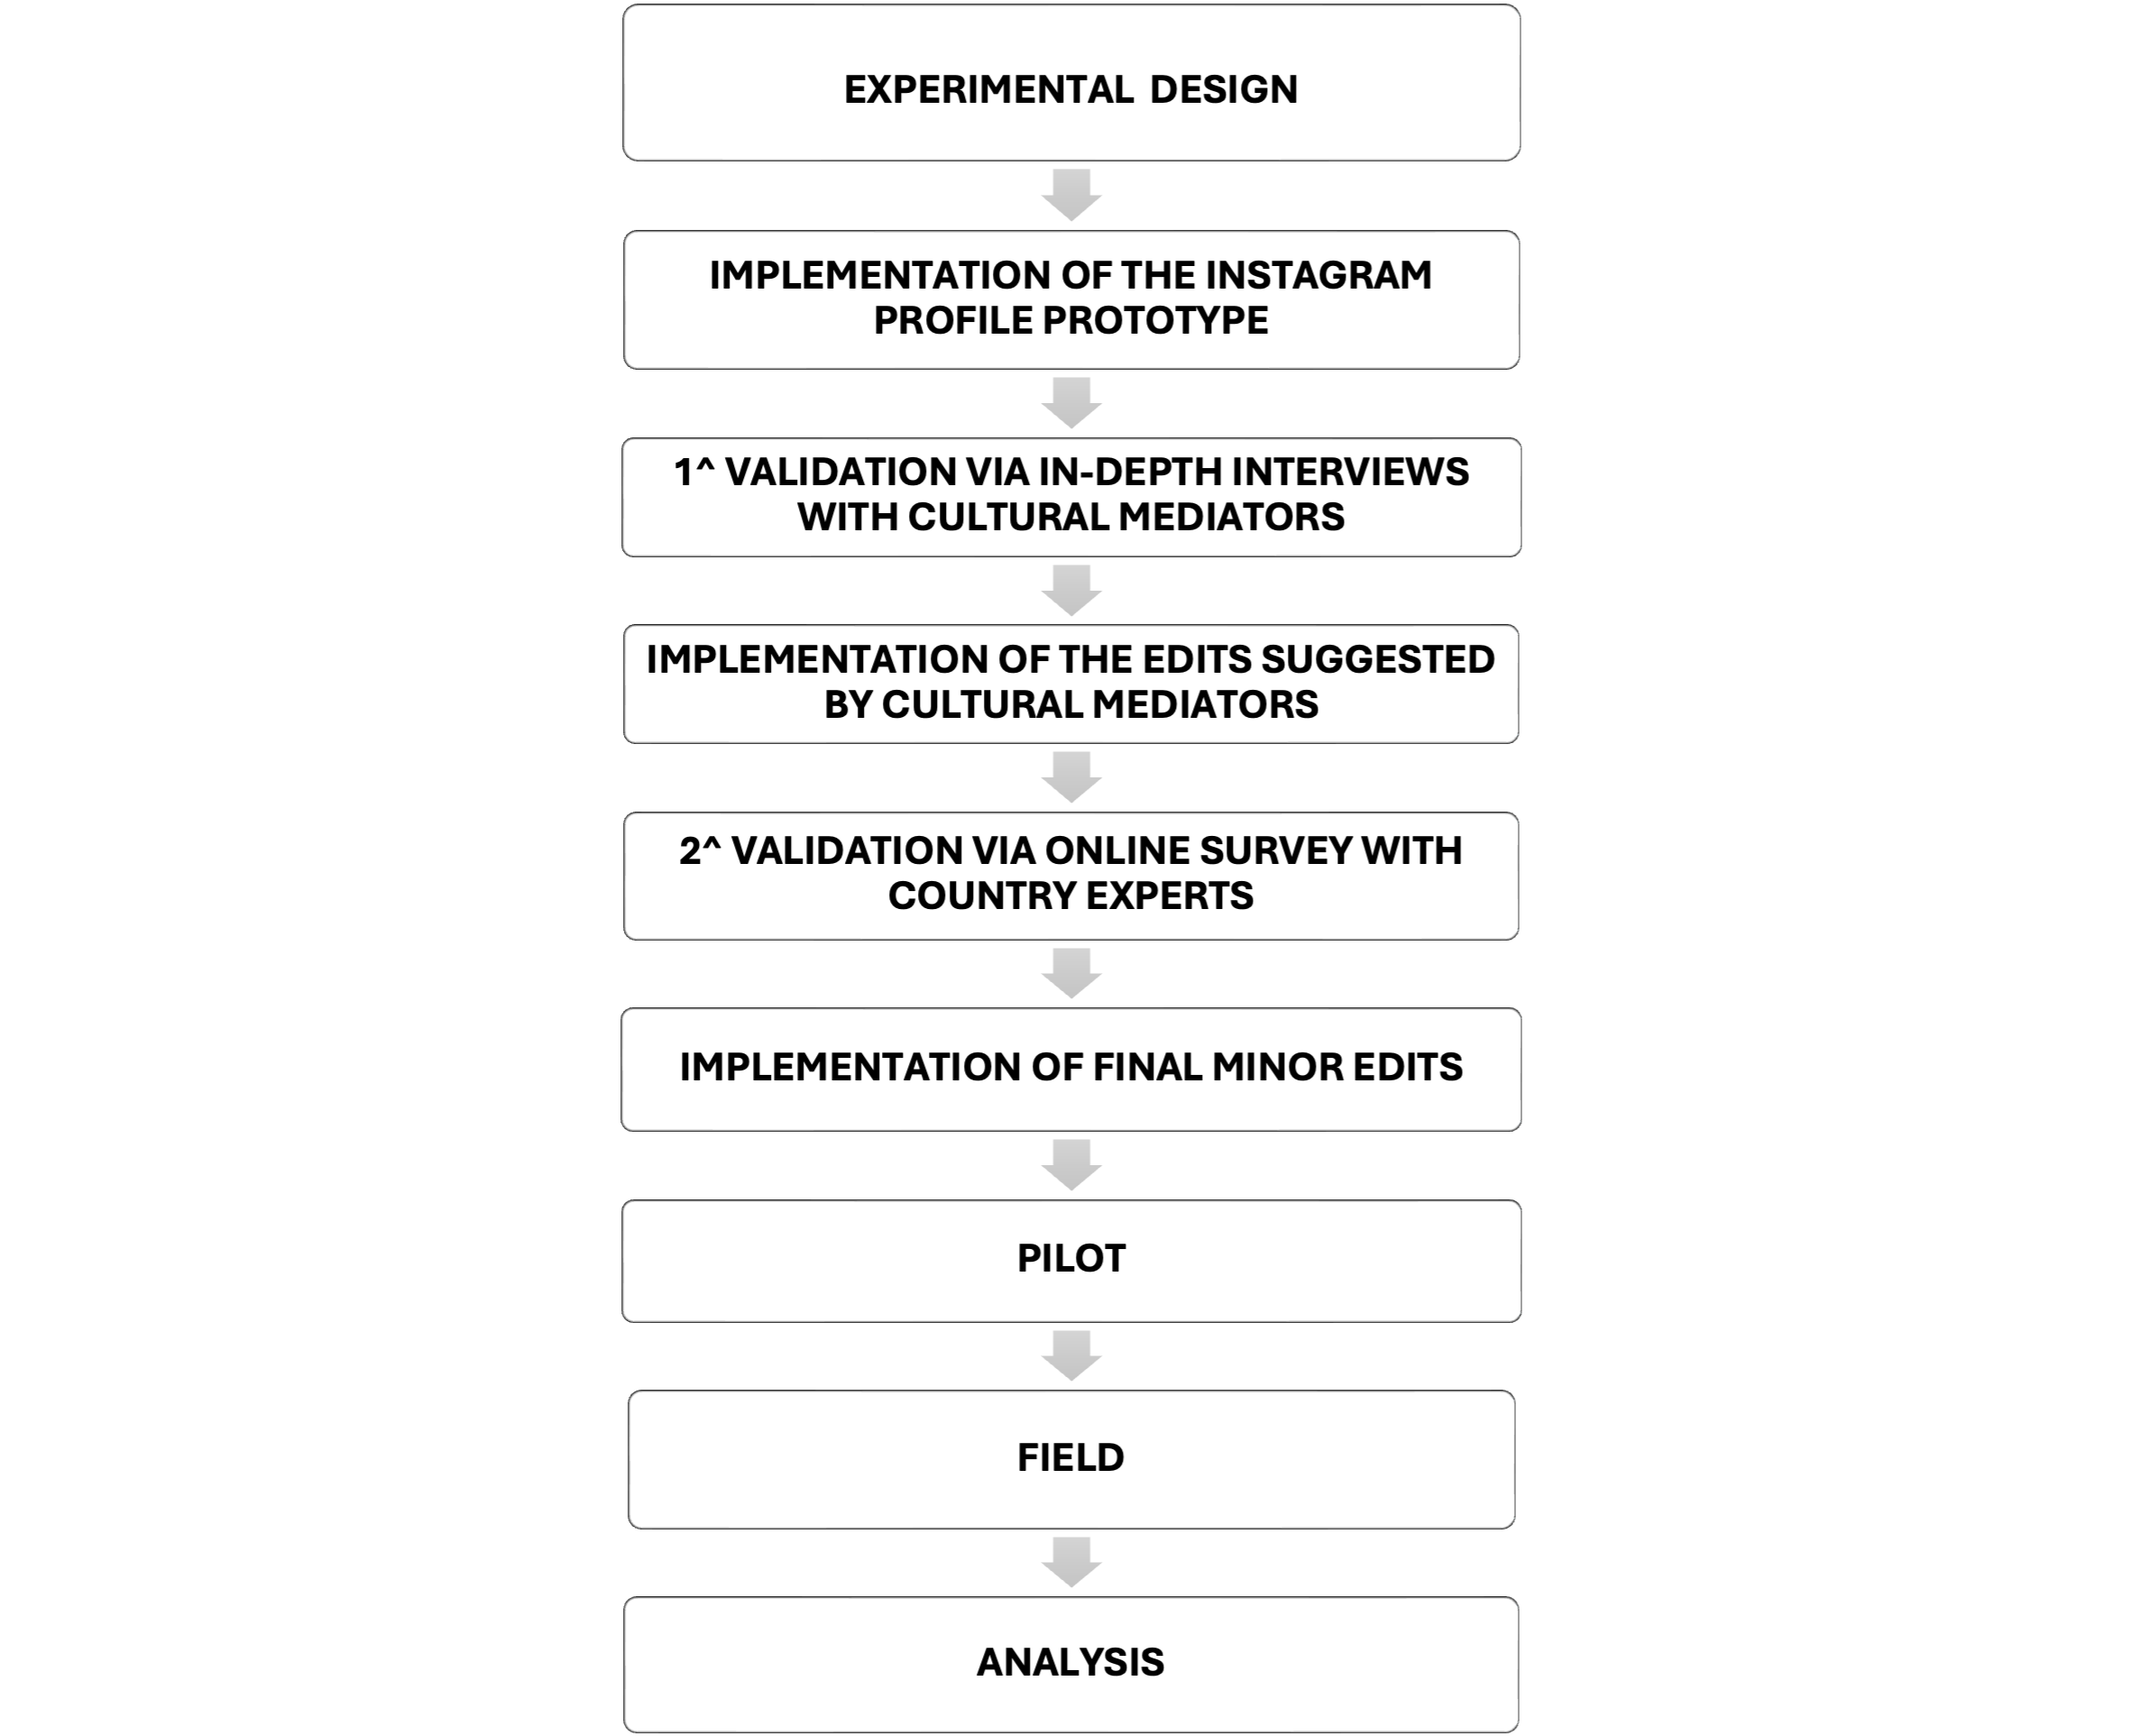
\includegraphics[width=0.9\linewidth]{Presentation/images/diagramma} \end{center}
\end{frame}

\begin{frame}{Methods: the visual conjoint experiment}
\phantomsection\label{methods-the-visual-conjoint-experiment}
\begin{block}{The data collection}
\phantomsection\label{the-data-collection}
\begin{itemize}
\tightlist
\item
  Survey fielded in Italy, France, Czech Republic, and Sweden in October
  2024 (Tot N=6000).
\item
  The data collection was conducted for the research project titled
  ``The Visual Politics of Populism'' (VIPOP).
\item
  In total, N=1500 individuals per country completed a CAWI
  questionnaire (representative sample in terms of age, gender, region
  and education).
\end{itemize}
\end{block}
\end{frame}

\begin{frame}{Methods: the visual conjoint experiment}
\phantomsection\label{methods-the-visual-conjoint-experiment-1}
\begin{block}{A visual conjoint approach}
\phantomsection\label{a-visual-conjoint-approach}
\begin{itemize}
\tightlist
\item
  The technique we employ is an evolution of the classical conjoint
  approach. The only difference is in how the stimulus is presented.
\item
  Participants see two pictures made from randomly extracted ``visual
  blocks''.
\item
  The pictures are created to resemble realistic Instagram profiles of
  politicians.
\item
  We chose Instagram for a series of reasons.

  \begin{itemize}
  \item
    It is one of the main platforms for online political communication
    (Larsson, 2021).
  \item
    Political actors behave as ``influencer politicians'' (Starita \&
    Trillò, 2022), displaying aspects of their private lives, their
    lifestyle choices, and their ``human side'' (Farkas \& Bene, 2021).
  \item
    The visual-centered nature of the platform made it a natural choice
    to exploit the potential of this design.
  \end{itemize}
\end{itemize}
\end{block}
\end{frame}

\begin{frame}{The empty template}
\phantomsection\label{the-empty-template}
\begin{center}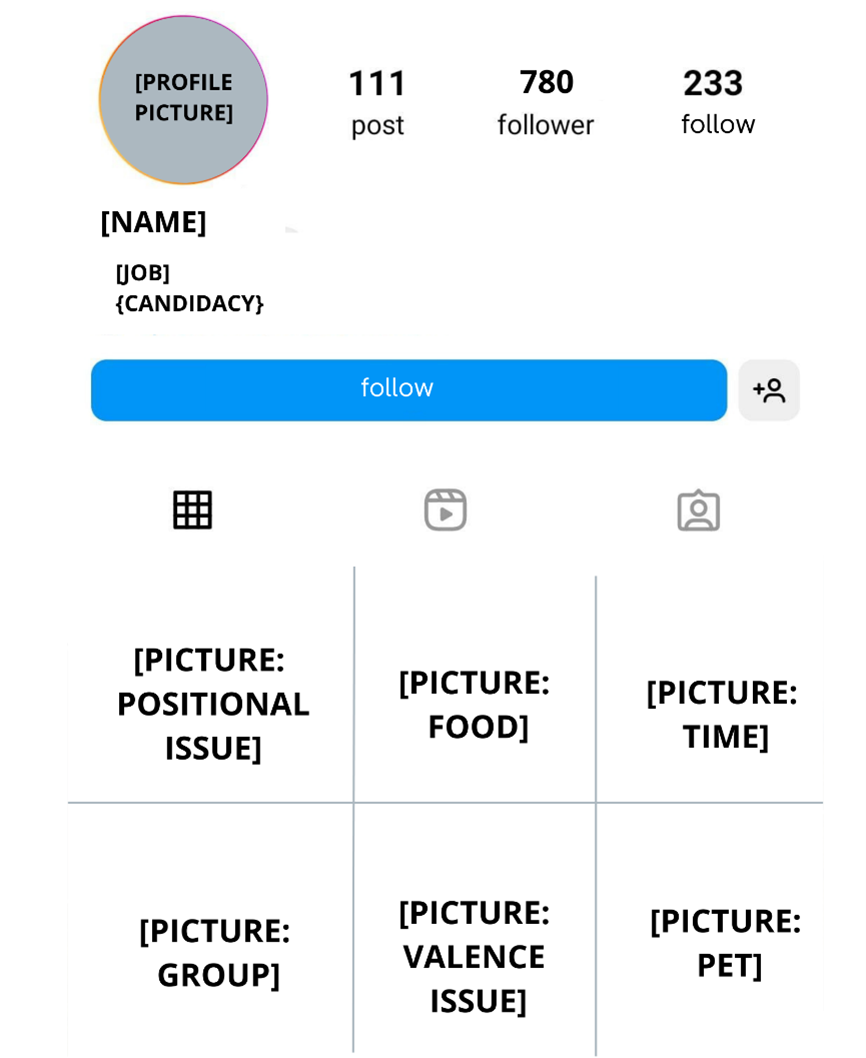
\includegraphics[width=0.5\linewidth]{../../visual_conjoint_experiment/Presentation/images/template} \end{center}
\end{frame}

\begin{frame}{Conjoint experiment procedure}
\phantomsection\label{conjoint-experiment-procedure}
\begin{itemize}
\tightlist
\item
  The profiles are generated through an R script employing the R package
  ``magick'' (Ooms, 2024).
\item
  Through this script, we generated 15.000 images per country.
\item
  For every conjoint task, two of these images were selected at random
  and shown to the respondents, keeping track of the specific features
  of every image to perform traditional conjoint analyses.
\item
  Every attribute is randomized uniformly,

  \begin{itemize}
  \tightlist
  \item
    Except for ethnicity, where the attribute level ``White'' has a
    probability of 0.95, ``Black'' of 0.05.
  \end{itemize}
\item
  Every respondent performs 5 tasks.

  \begin{itemize}
  \tightlist
  \item
    For each task, the respondents are asked which one of the two
    politicians they consider more right-wing.
  \end{itemize}
\end{itemize}
\end{frame}

\begin{frame}{The visual attributes 1}
\phantomsection\label{the-visual-attributes-1}
\begin{center}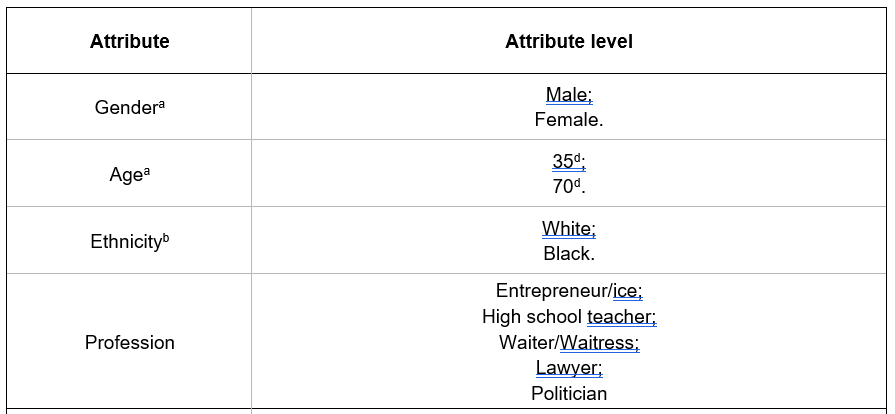
\includegraphics[width=0.95\linewidth]{../../visual_conjoint_experiment/Presentation/images/attributes1} \end{center}

Names have been selected among the 5 most popular in each country,
according to official statistical institutes, and further validated by
AI and our cultural mediators. For black politicians, we selected names
among the Senegal community, as this country-origin ranks high among
African immigrants in selected countries.
\end{frame}

\begin{frame}{The profile pics}
\phantomsection\label{the-profile-pics}
\begin{center}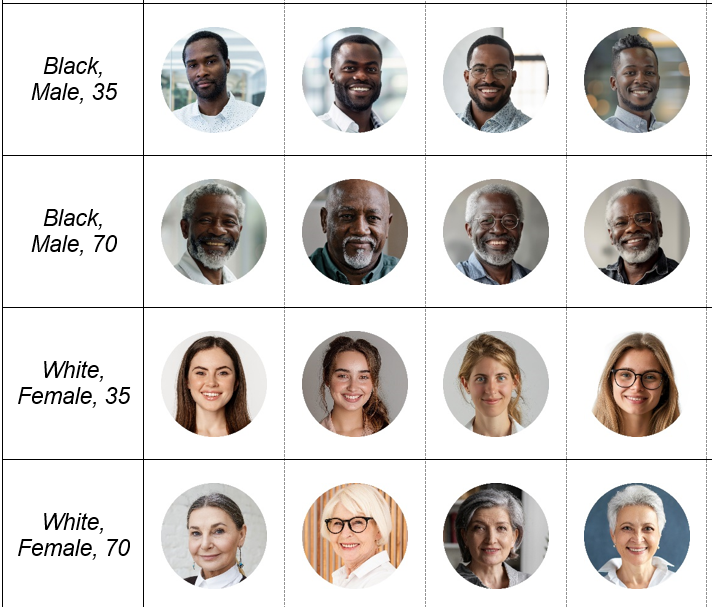
\includegraphics[width=0.95\linewidth]{../../visual_conjoint_experiment/Presentation/images/attributes2} \end{center}
\end{frame}

\begin{frame}{The visual attributes 2}
\phantomsection\label{the-visual-attributes-2}
\begin{center}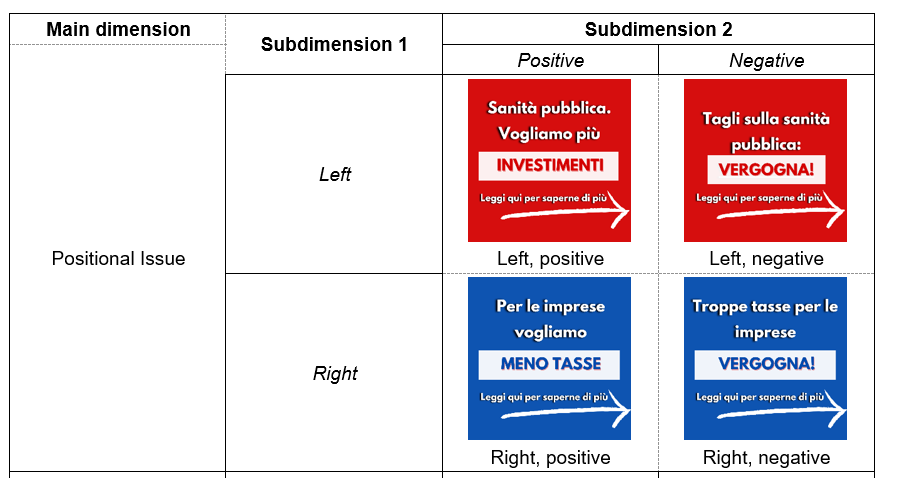
\includegraphics[width=0.95\linewidth]{../../visual_conjoint_experiment/Presentation/images/attributes3} \end{center}
\end{frame}

\begin{frame}{The visual attributes 3}
\phantomsection\label{the-visual-attributes-3}
\begin{center}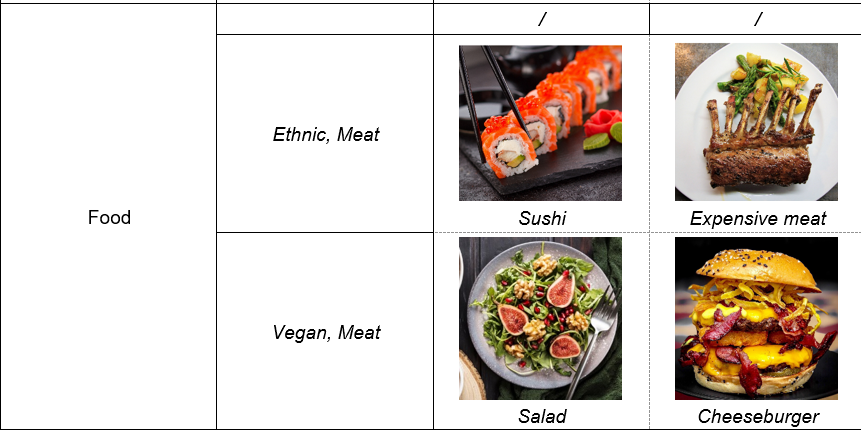
\includegraphics[width=0.95\linewidth]{../../visual_conjoint_experiment/Presentation/images/attributes4} \end{center}
\end{frame}

\begin{frame}{The visual attributes 4}
\phantomsection\label{the-visual-attributes-4}
\begin{center}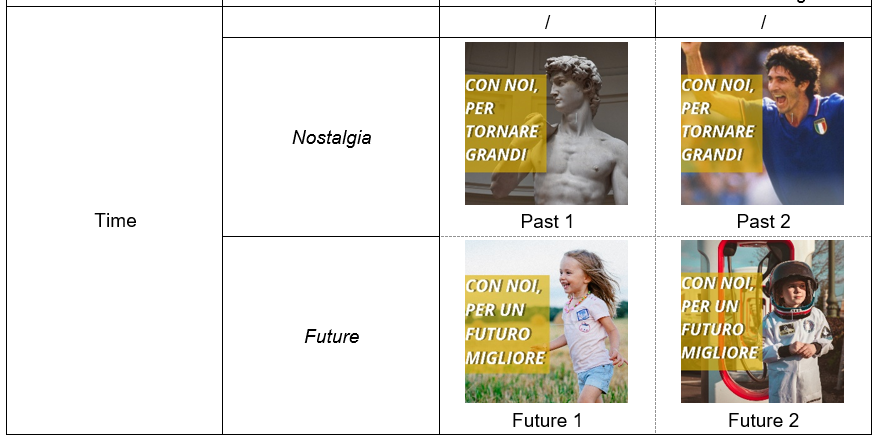
\includegraphics[width=0.95\linewidth]{../../visual_conjoint_experiment/Presentation/images/attributes5} \end{center}
\end{frame}

\begin{frame}{The visual attributes 5}
\phantomsection\label{the-visual-attributes-5}
\begin{center}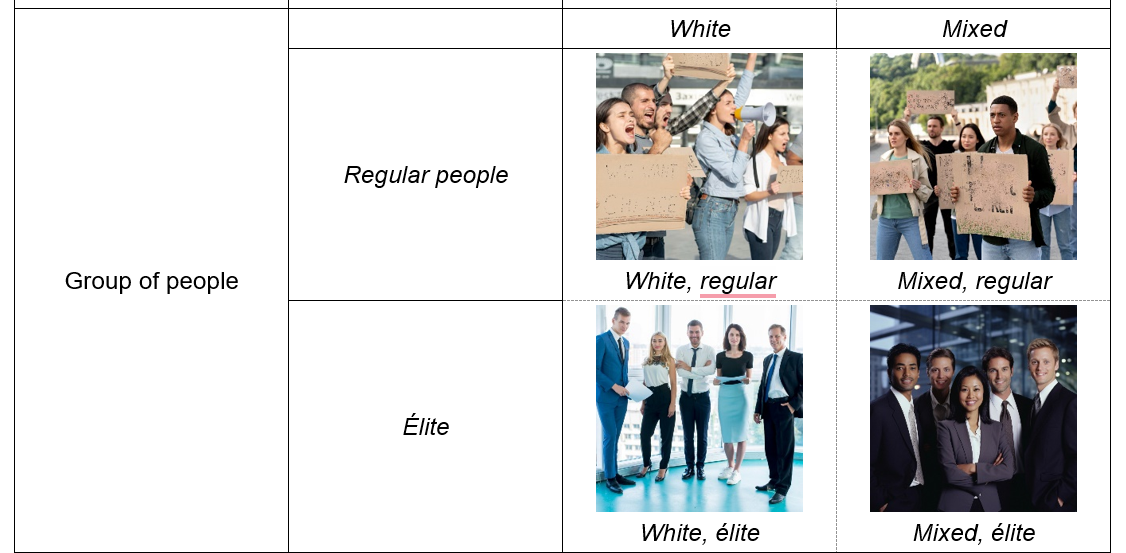
\includegraphics[width=0.95\linewidth]{../../visual_conjoint_experiment/Presentation/images/attributes6} \end{center}
\end{frame}

\begin{frame}{The visual attributes 6}
\phantomsection\label{the-visual-attributes-6}
\begin{center}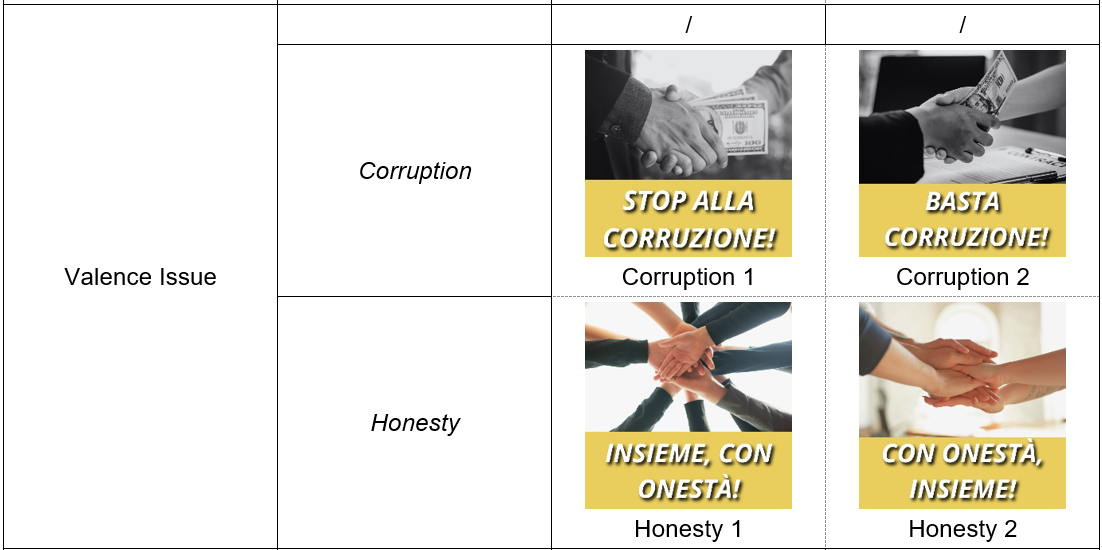
\includegraphics[width=0.95\linewidth]{../../visual_conjoint_experiment/Presentation/images/attributes8} \end{center}
\end{frame}

\begin{frame}{The visual attributes 7}
\phantomsection\label{the-visual-attributes-7}
\begin{center}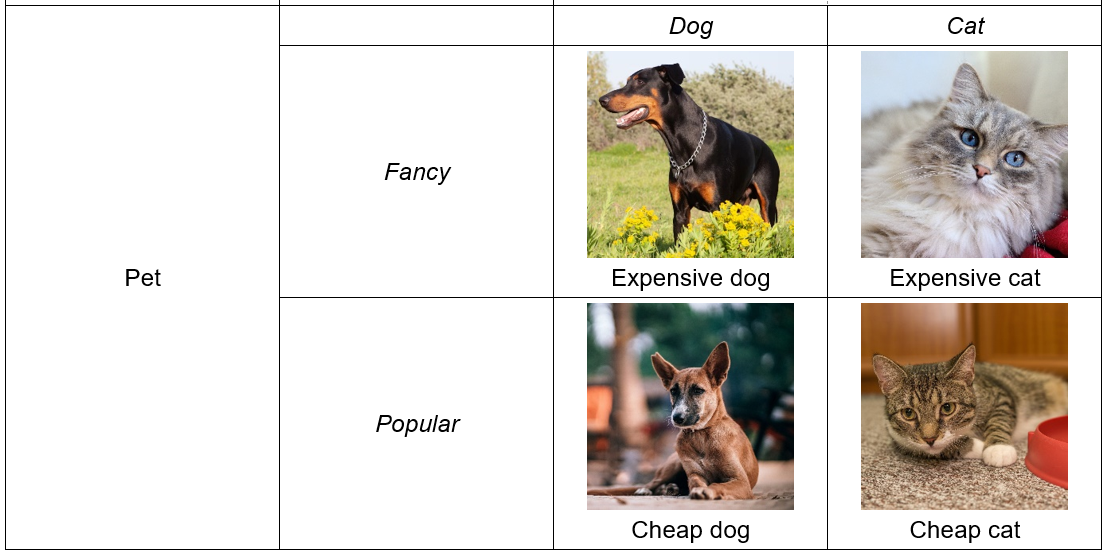
\includegraphics[width=0.95\linewidth]{../../visual_conjoint_experiment/Presentation/images/attributes7} \end{center}
\end{frame}

\begin{frame}{The filled templates: examples 1}
\phantomsection\label{the-filled-templates-examples-1}
\begin{center}
\includegraphics[width=0.49\linewidth]{../../visual_conjoint_experiment/Presentation/images/IT/ex1} 
\includegraphics[width=0.49\linewidth]{../../visual_conjoint_experiment/Presentation/images/IT/ex2} \end{center}
\end{frame}

\begin{frame}{The filled templates: examples 2}
\phantomsection\label{the-filled-templates-examples-2}
\begin{center}
\includegraphics[width=0.49\linewidth]{../../visual_conjoint_experiment/Presentation/images/IT/ex3} 
\includegraphics[width=0.49\linewidth]{../../visual_conjoint_experiment/Presentation/images/IT/ex4} \end{center}
\end{frame}

\begin{frame}{Analyses}
\phantomsection\label{analyses}
We are interested in showing how much each attribute level leads to
inferring that someone is ideologically right-(or left-)wing or
populist.

In light of recent criticisms of the AMCE as an estimator for certain
type of conjoint outcomes (Leeper et al., 2020; Ganter 2021), we will
present the results relating to the dichotomous outcome with MMs.

Unfortunately, due to delays with the data collection, we are now only
able to present results on the Italian pilot (N=150).
\end{frame}

\begin{frame}{Preliminary results}
\phantomsection\label{preliminary-results}
\begin{center}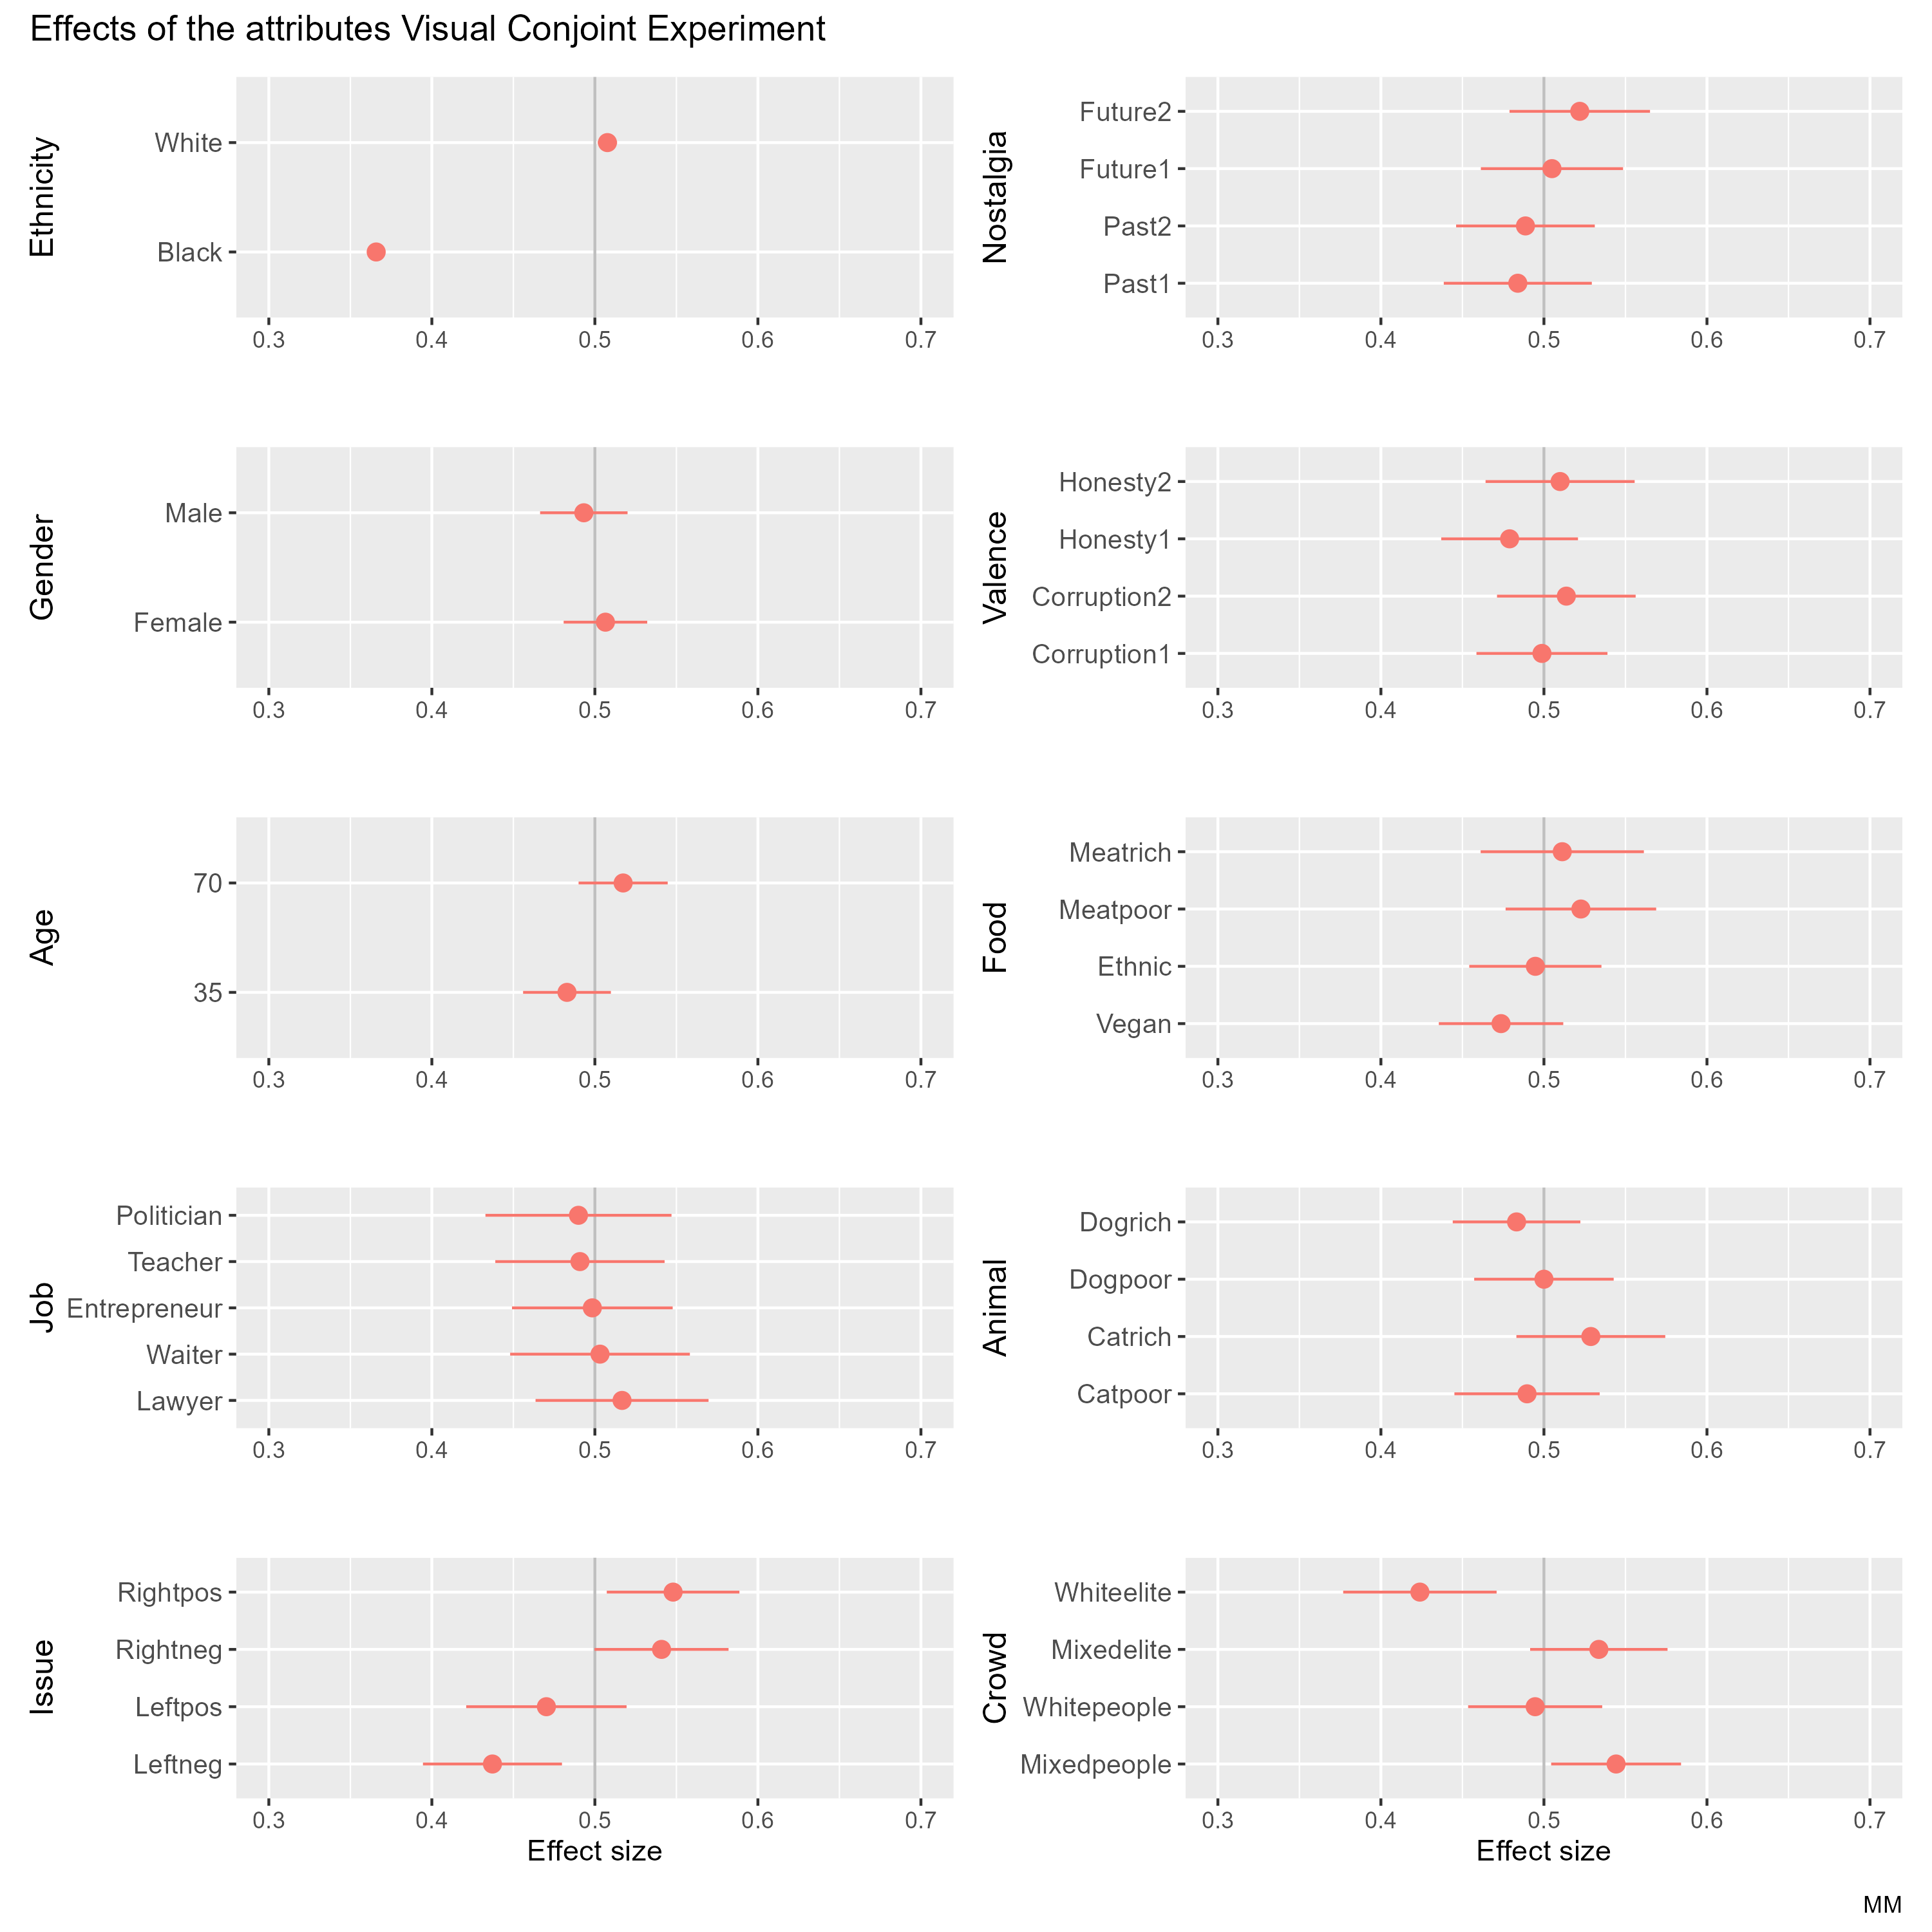
\includegraphics[width=0.7\linewidth]{Presentation/images/singlecountry} \end{center}
\end{frame}

\begin{frame}{Preliminary results}
\phantomsection\label{preliminary-results-1}
\begin{center}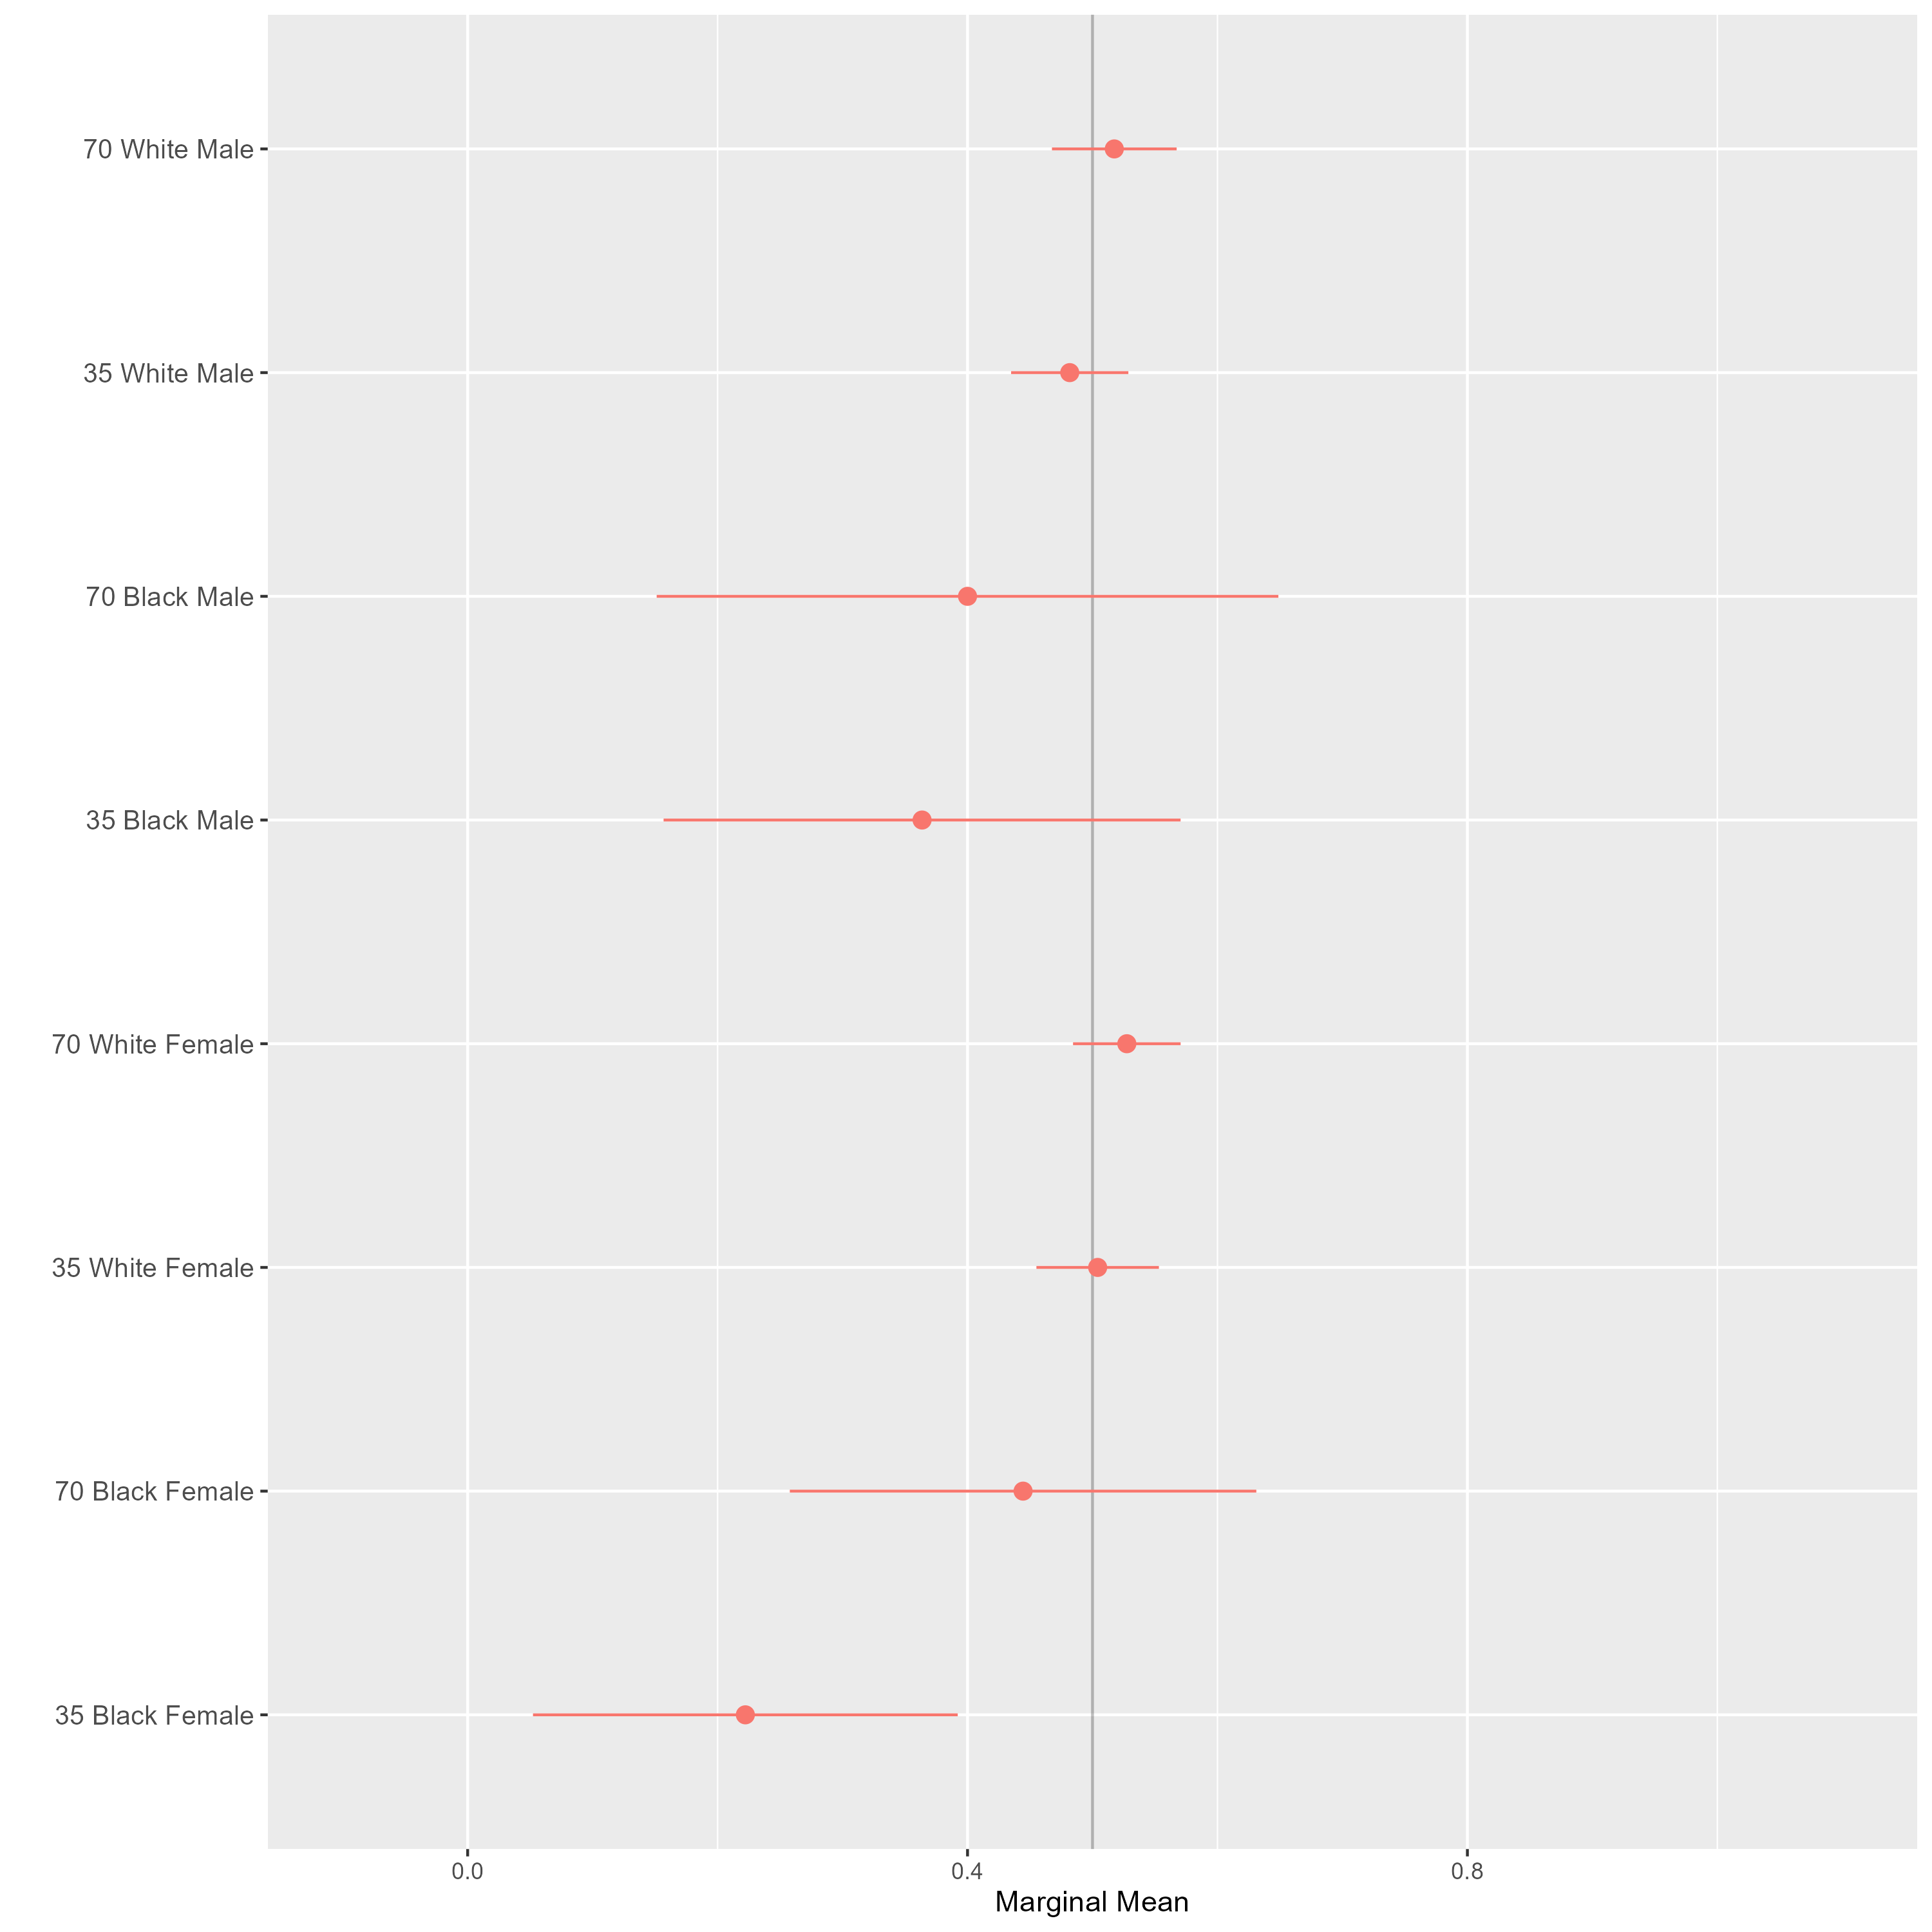
\includegraphics[width=0.75\linewidth]{Presentation/images/interaction1} \end{center}
\end{frame}

\begin{frame}{Preliminary results}
\phantomsection\label{preliminary-results-2}
\begin{center}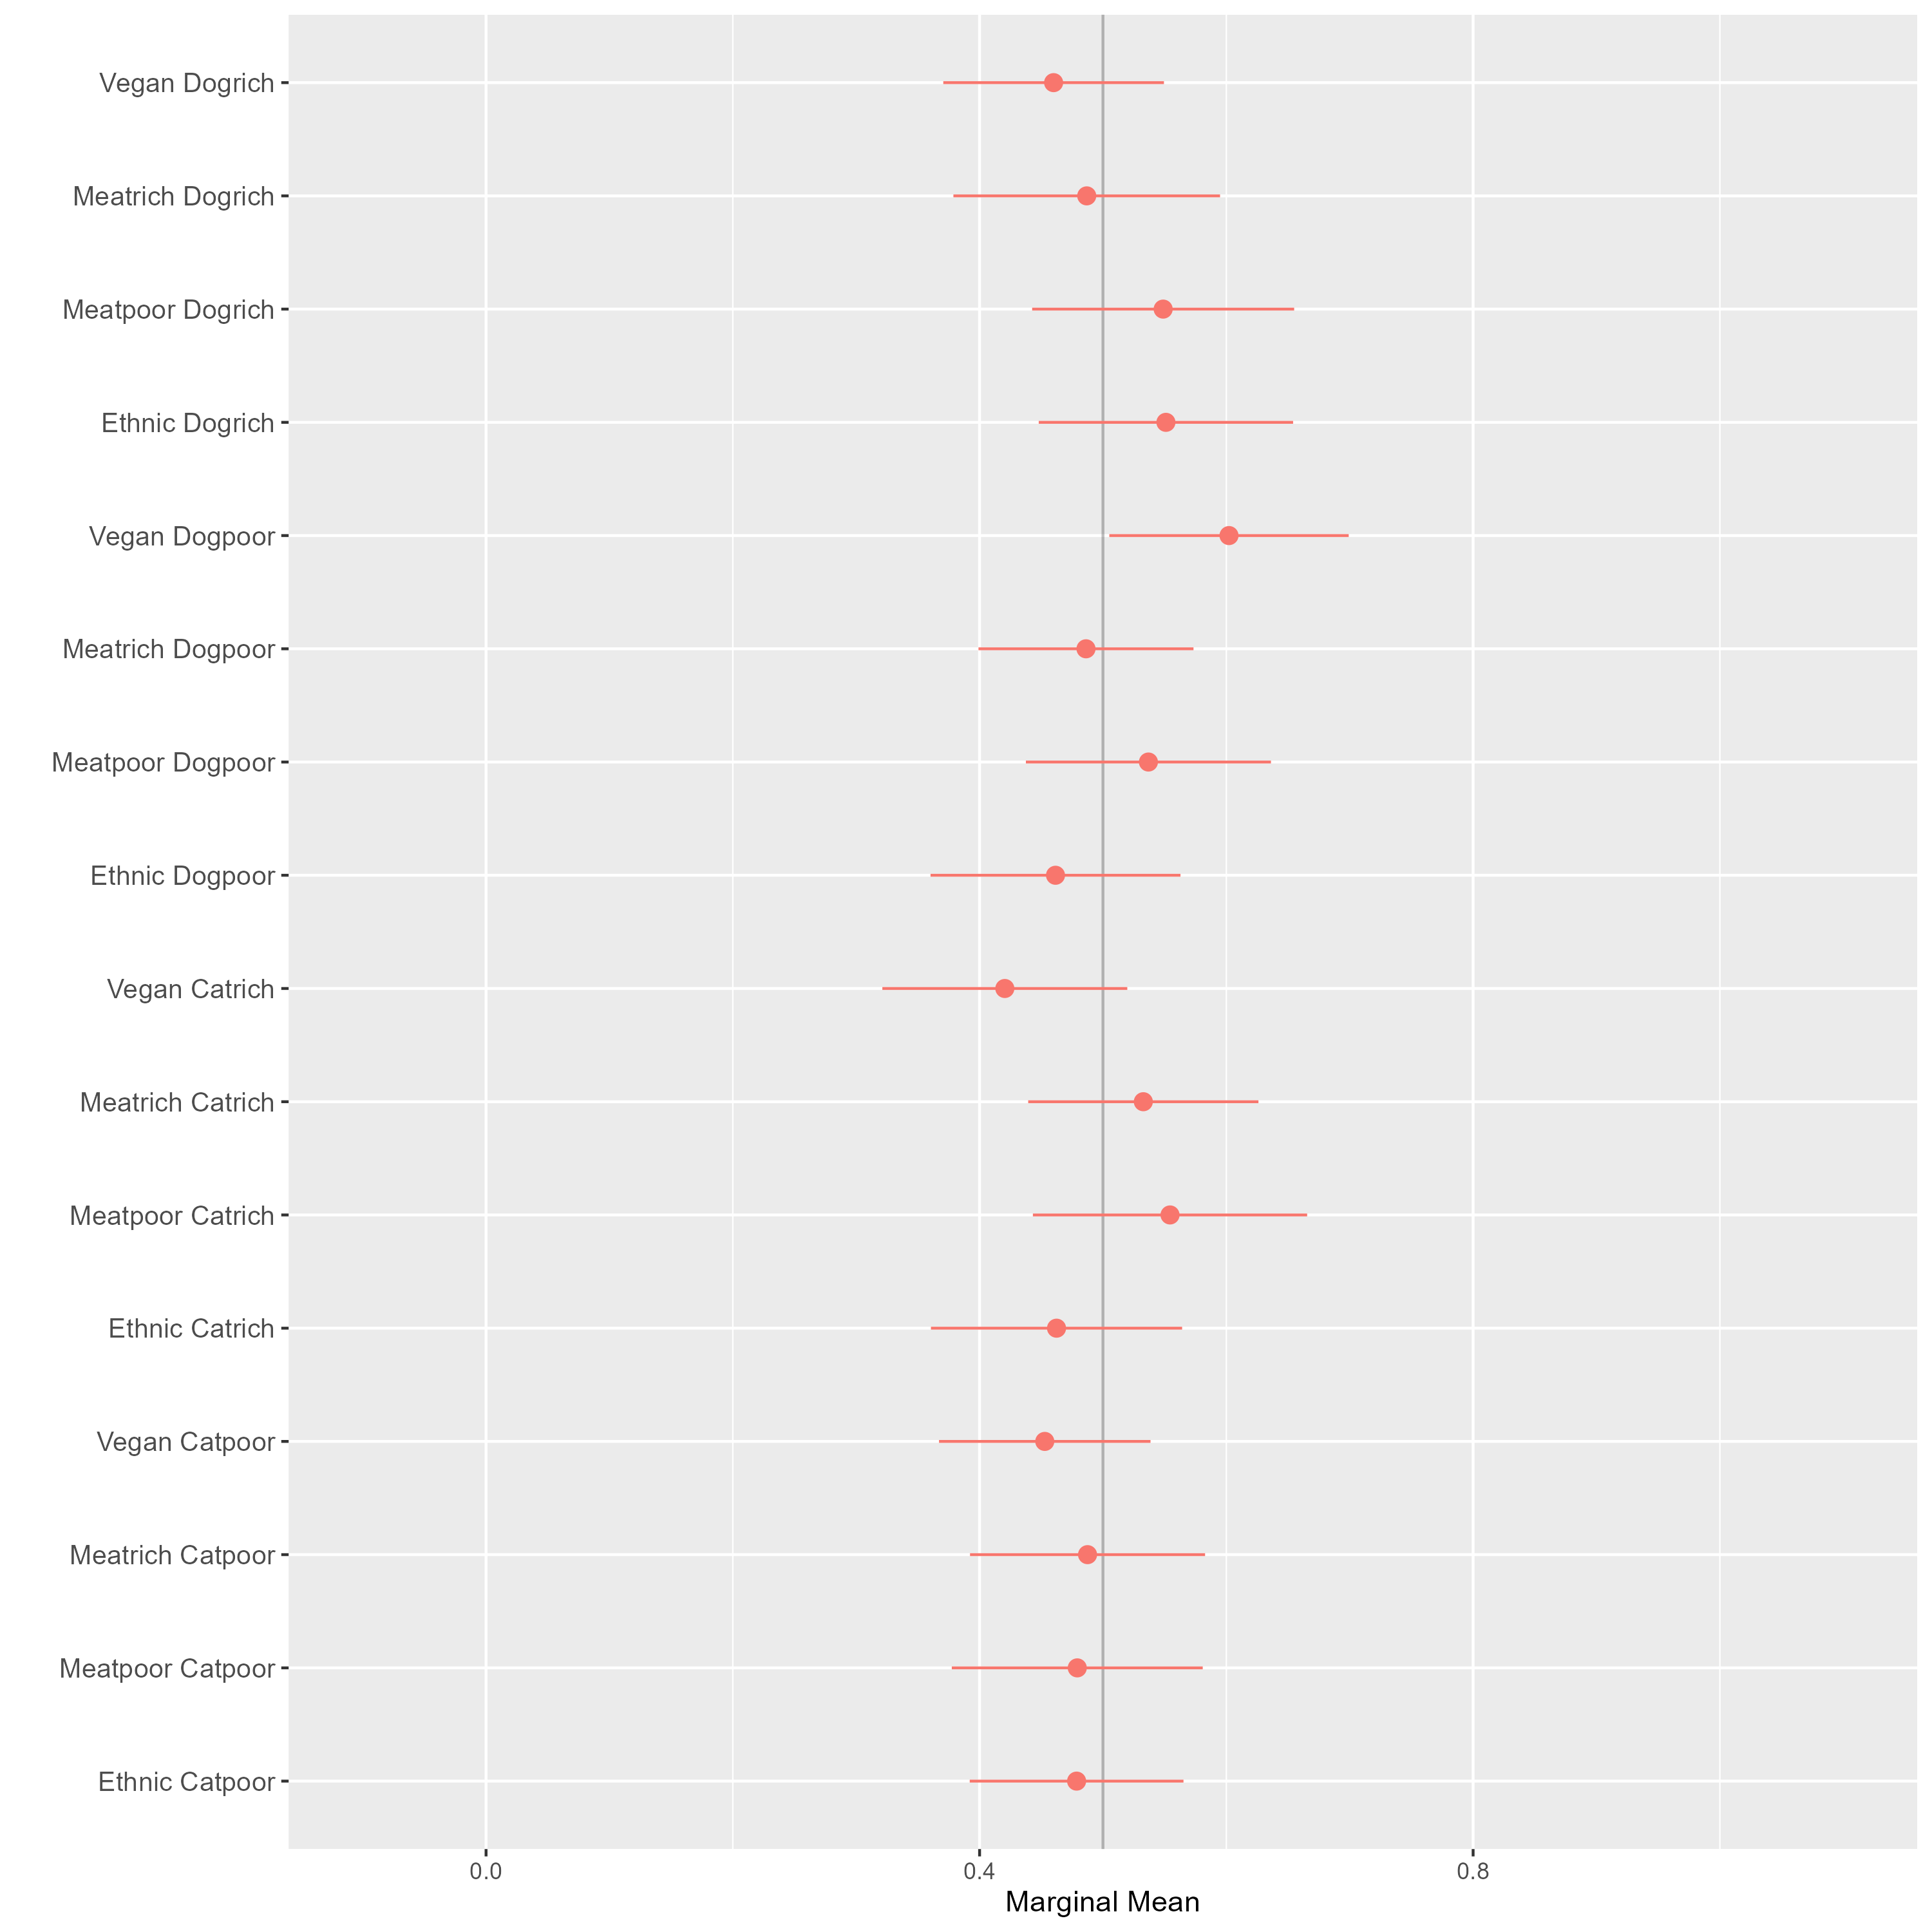
\includegraphics[width=0.75\linewidth]{Presentation/images/interaction2} \end{center}
\end{frame}

\begin{frame}{Preliminary results}
\phantomsection\label{preliminary-results-3}
\begin{center}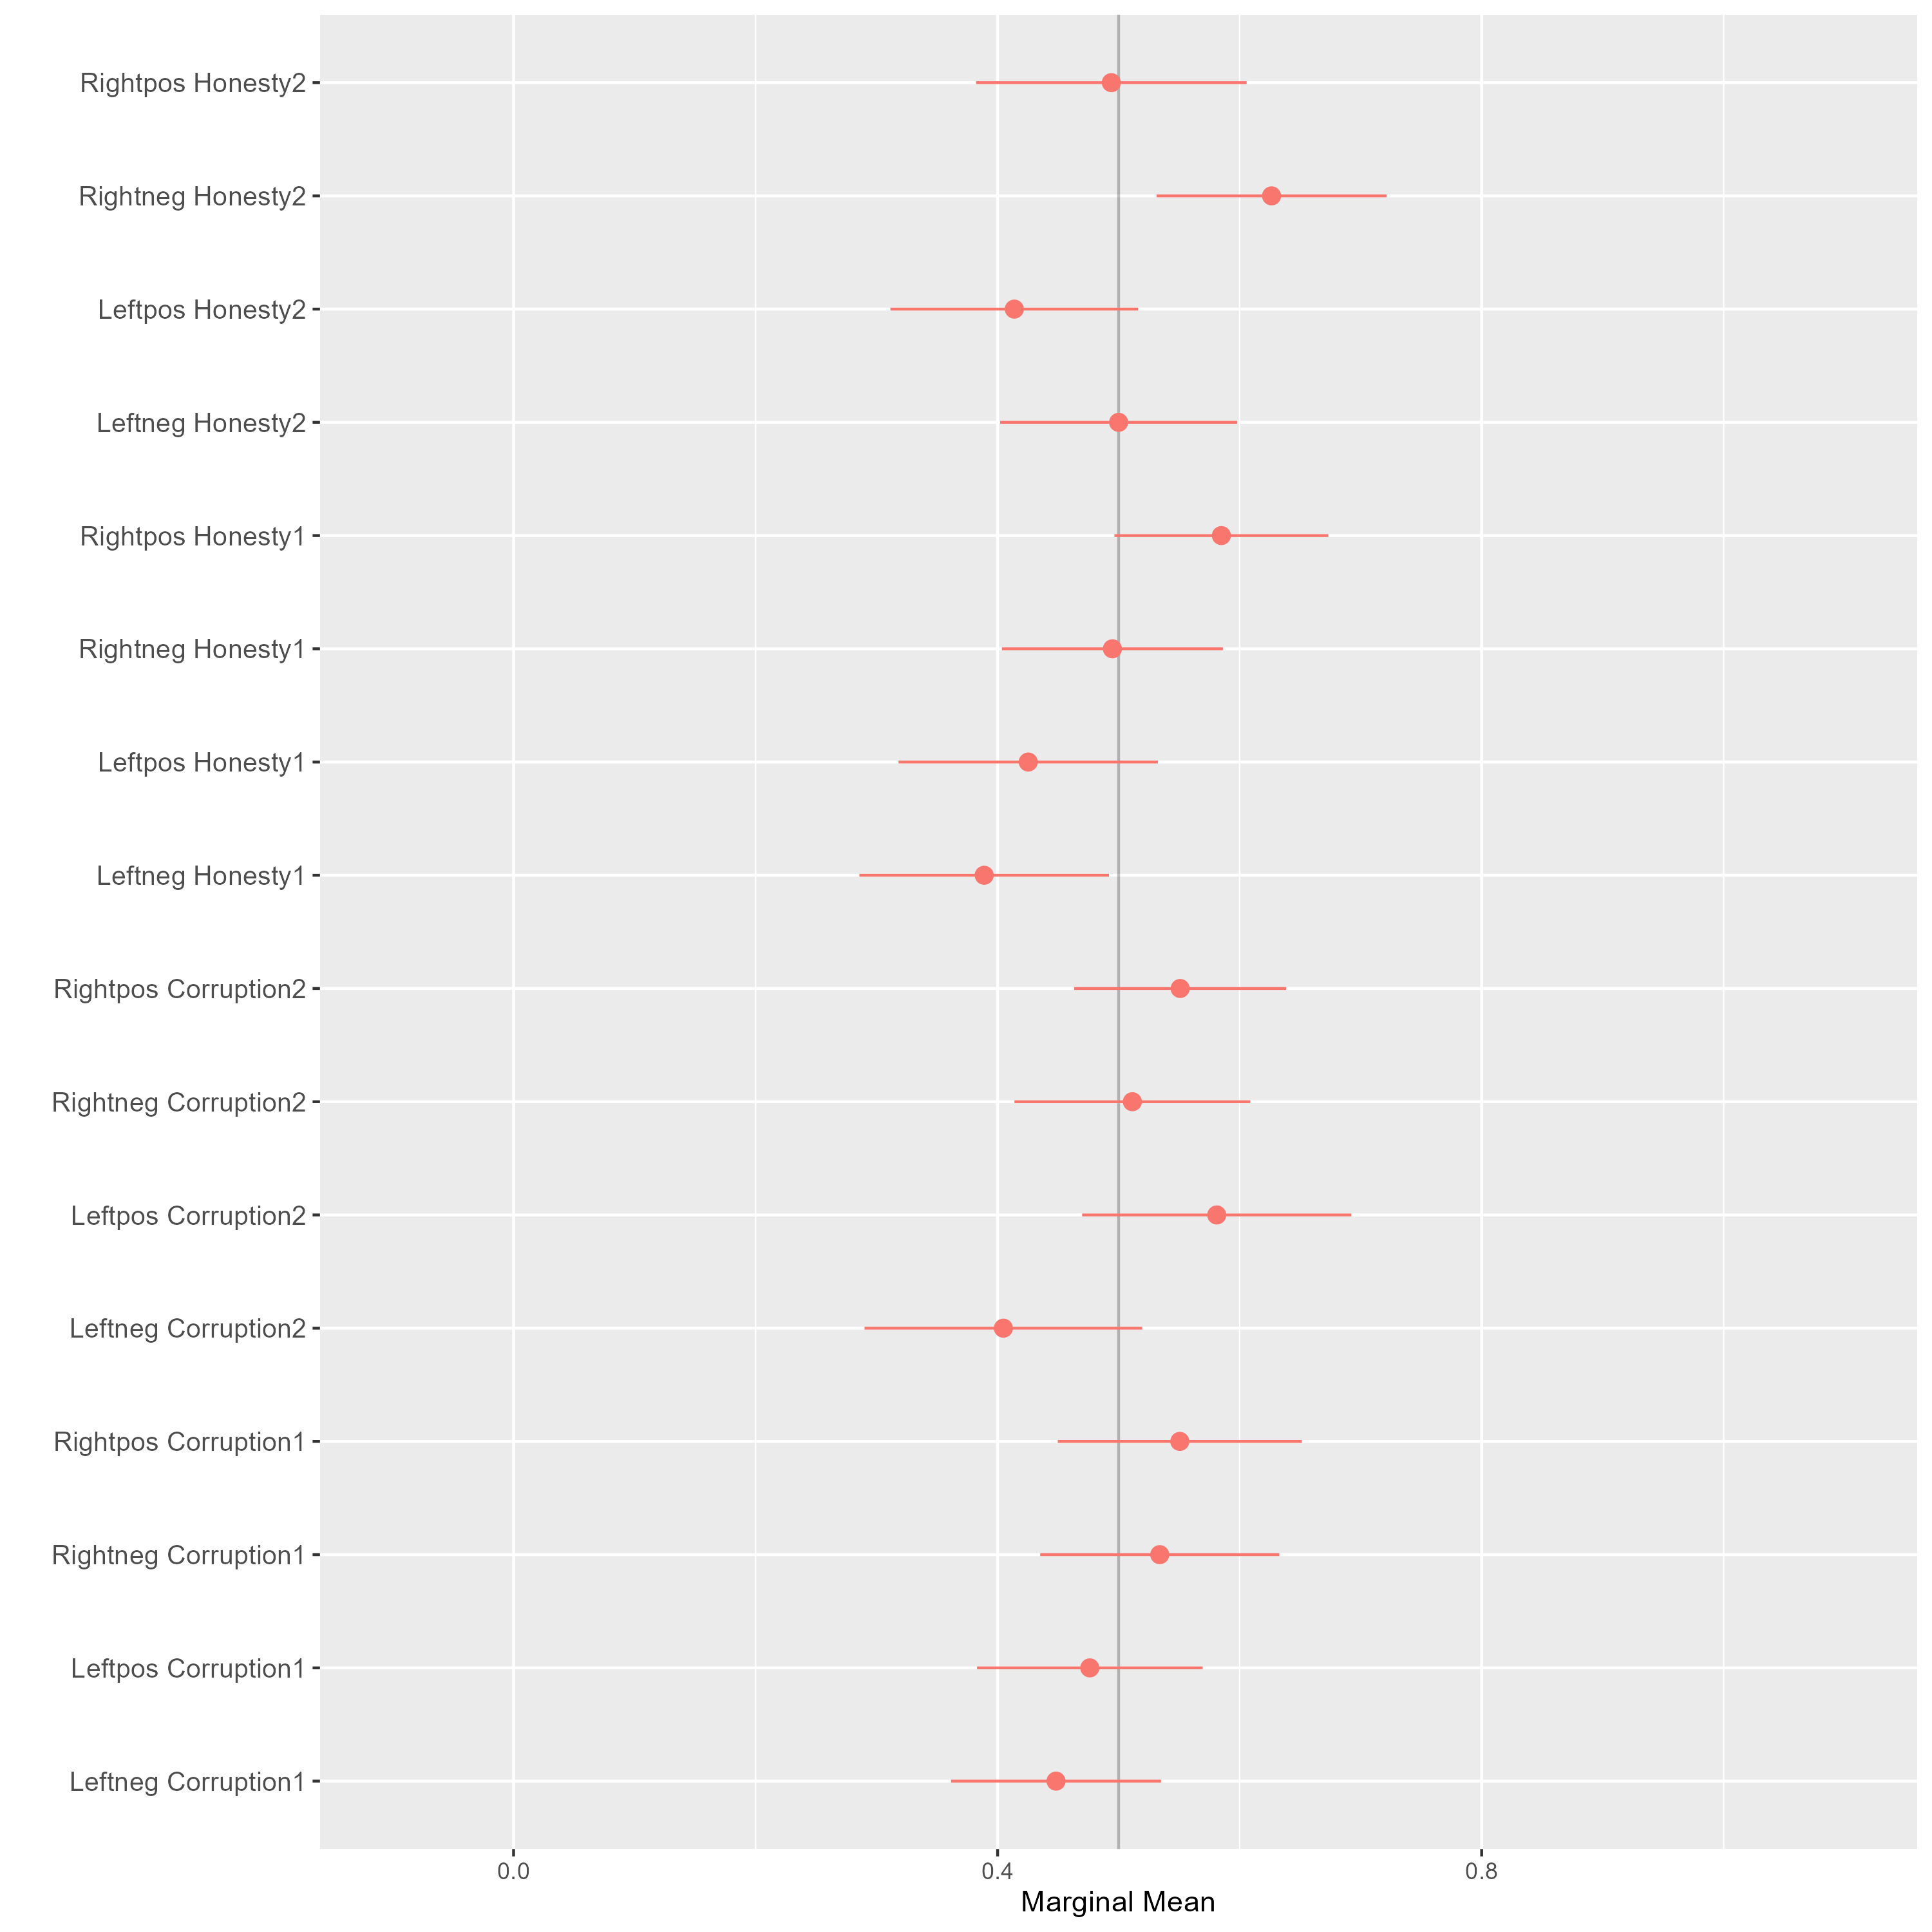
\includegraphics[width=0.75\linewidth]{Presentation/images/interaction3} \end{center}
\end{frame}

\begin{frame}{Preliminary conclusions}
\phantomsection\label{preliminary-conclusions}
\begin{itemize}
\item
  \textbf{The political wins over the apolitical:} based on these pilot
  results, we have reasons to believe that, in presence of political
  cues, the role of apolitical cues becomes marginal.
\item
  Yet, especially for sociodemographic cues, it seems to be reason to
  believe that they indeed keep being relevant.
\item
  Overall, the visual conjoint design promises to be an important
  euristic tool for future research endeavors.
\end{itemize}
\end{frame}

\begin{frame}{Thank you!}
\phantomsection\label{thank-you}
\begin{center}\includegraphics[width=1\linewidth]{../../../Papers and Chapters/ViPop2024/EUTextVis1/report/images/thankyou} \end{center}
\end{frame}

\end{document}
